% % !TEX root = ../TAMU_Thesis_Main.tex

% %%%%%%%%%%%%%%%%%%%%%%%%%%%%%%%%%%%%%%%%%%%%%%%%%%%%%%%%%%%%%%%%%%%%%%
% %%                           APPENDIX B
% %%%%%%%%%%%%%%%%%%%%%%%%%%%%%%%%%%%%%%%%%%%%%%%%%%%%%%%%%%%%%%%%%%%%%
\chapter{Appendix for Numerical mixing suppresses submesoscale baroclinic instabilities over sloping bathymetry}%\label{appendix:01}
\section{Ensemble of near-inertial wind amplitude} 

\begin{figure}[t]
    \begin{center}
    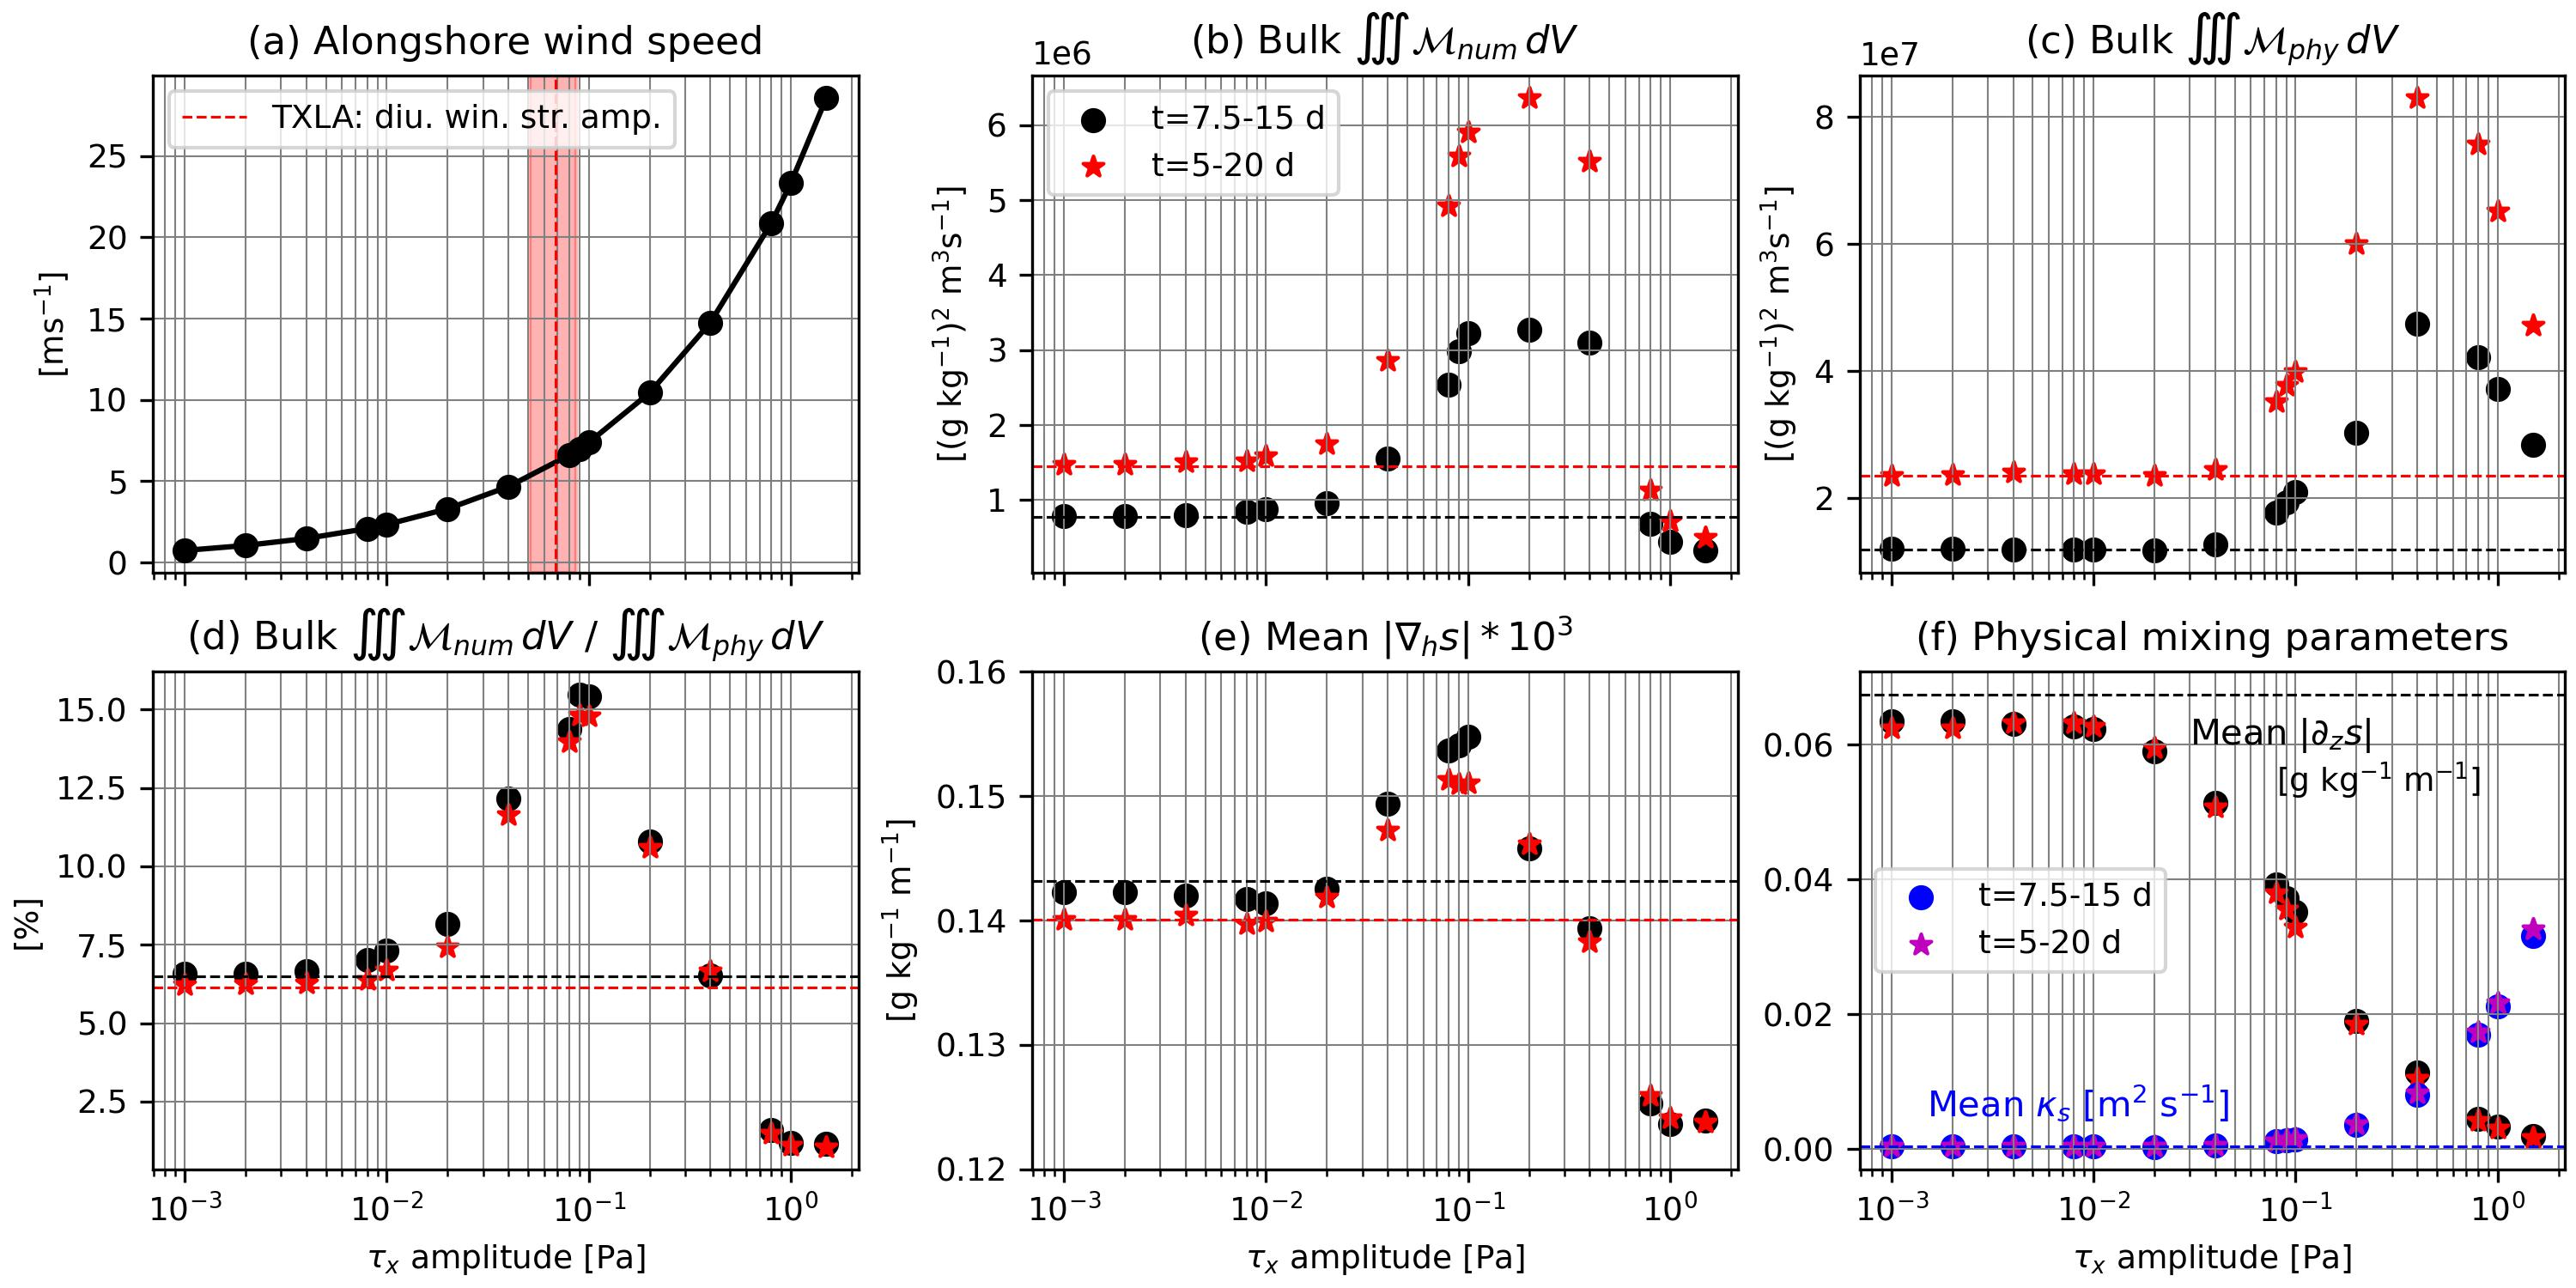
\includegraphics[width = \linewidth]{figures/shelfstrat_2024/mixing_function_taux.jpg}\\
    \caption{(a) Wind speed as a function of $\tau_0^x$ calculated using Eq. \ref{eqn:windspd}, with each dot representing a different numerical simulation. The amplitude of the diurnal wind stress magnitude spatially- and temporally averaged for the entire realistic simulation of the child domain \citep[see Fig. 7 a of] []{Schlichting23} with 95\% confidence intervals is shown with the red dashed line and shaded areas. Bulk $\mathcal{M}_{num}$ (b) and $\mathcal{M}_{phy}$ (c). (d) Ratio of bulk $\mathcal{M}_{num}$ to $\mathcal{M}_{phy}$ expressed expressed as a percent. Spatially- and temporally-averaged $|\nabla_h s|$ (e), $|\partial_z s|$ (f), and $\kappa_v$ (f). Quantities in (b)-(f) are calculated in the initially stratified region for two time periods and the horizontal dashed lines show unforced case values for their respective time periods coded by color.} \label{fig:wind_ensembles}
     \end{center}
\end{figure}

The impacts of varying the near-inertial alongshore wind stress amplitude $\tau_0^x$ on bulk mixing quantities associated with each ensemble member are shown in Fig. \ref{fig:wind_ensembles}. In addition, we show spatially- and temporally averaged parameters related to each mixing quantity to better understand how the bulk mixing quantities change in response to different $\tau_0^x$. To provide a sense of scale for $\tau_0^x$, we plot the amplitude of the wind speed $U_{wind}$ by solving the equation
\begin{equation} \label{eqn:windspd}
    \tau_0^x=\rho_a C_d U_{wind}^2 \, ,
\end{equation}
where $\rho_a$ is the density of air and $C_d$ is the drag coefficient set to a constant value of 0.0015. $U_{wind}$ of the ensemble runs span from $<1$ms$^{-1}$ to tropical storm force winds (29 ms$^{-1}$, until the model blew up). 

All bulk quantities are shown from days 5-20 and days 7.5-15 to indicate the trends are robust. The x-axes are on a log$_{10}$ scale. The time-averaged amplitude of the diurnal (inertial) wind stress magnitude from the realistic model \citep[Fig. 7 a of ][]{Schlichting23} is shown to contextualize the base case. The base case wind is slightly more energetic than the mean values observed during the realistic model simulation. The realistic surface forcing is highly variable, but spatially-averaged values rarely exceeded 10 ms$^{-1}$. 

$\tau_0^x$ values from $10^{-3}-10^{-2}$ Pa have little impact on volume-integrated $\mathcal{M}_{num}$ (Fig. \ref{fig:wind_ensembles} b) or $\mathcal{M}_{phy}$ (Fig. \ref{fig:wind_ensembles} c). As $\tau_0^x$ increases, $\mathcal{M}_{num}$ rapidly grows until plateauing from $\tau_0^x$=0.1-0.3 Pa, then rapidly decreases. In linear space, this qualitatively resembles a Chi-squared distribution with few degrees of freedom such that the peak is biased towards zero. The time- and spatially-averaged $|\nabla_h s|$ peaks at 0.1 Pa then begins to rapidly decrease (Fig. \ref{fig:wind_ensembles} e). As the wind stress amplitude approaches 1 Pa, winds suppress the instabilities, causing $\mathcal{M}_{num}$ to decrease. For example, strong winds create pulses over the ocean surface (not shown). A background $|\nabla_h s|$ is still maintained because fronts are not allowed to form and there is not explicit lateral mixing. 

Volume-integrated $\mathcal{M}_{num}$ is more sensitive to the winds relative to $\mathcal{M}_{phy}$. $\mathcal{M}_{num}$ peaks at 0.1 Pa and $\mathcal{M}_{phy}$ peaks at 0.4 Pa. As the near-inertial wind amplitude increases, the instabilities are eventually suppressed while the water column continues to be vertically mixed. The parameters governing $\mathcal{M}_{phy}$ are shown in Fig. \ref{fig:wind_ensembles} (f). The magnitude of the time-and spatially-averaged averaged vertical salinity gradient $|\partial_z s|$ exhibits an inverse sigmoid relationship with $\tau_0^x$. For ensemble runs with the largest $\tau_0^x$, instabilities are entirely suppressed and wind mixing reduces $|\partial_z s|$ to nill. The mean vertical eddy diffusivity $\kappa_v$ exhibits exponential growth. The increased growth of $\mathcal{M}_{phy}$ despite the decrease in $|\partial_z s|$ highlights the covariance between $\kappa_v$ and $|\partial_z s|$. 
% \chapter{A Second Appendix Whose Title Is Much Longer Than The First}\label{appendix:02}

% Text for the Appendix follows.

% \begin{figure}[h]
% \centering
% 
\includegraphics[scale=.50]{figures/Penguins.jpg}
% \caption{Another TAMU figure.}
% \label{fig:tamu-fig6}
% \end{figure}

% \section{Appendix Section}

% \section{Second Appendix Section}